\Gls{ml} has become an important sub-field of computer science. It emulates human-like learning using mathematical models, so predictions can be made about new data in the future. Rather than explicitly programming how to make those predictions, the developer provides sample data during \textit{training}. Once the accuracy of the trained model is sufficient, it can be used for \textit{inference}. The model can be thought of as the approximation of a function mapping from the input data to some output, e.g., a label for classification, or a numerical value for regression~\cite[p.~164]{IanGoodfellow.2016}.

\section{Artificial Neural Networks}
While there are a variety of \gls{ml} models in use today, \glspl{ann} are among the most powerful and flexible, due to their ability to represent complex functions~\cite[p.~163]{IanGoodfellow.2016}. They find application in fields as diverse as image and speech recognition, movie recommendations and medical diagnosis.

\Glspl{ann} are composed of multiple layers, with the output of one layer being the input of another layer. The first layer receives the input data, and the last layer produces the final output. With an increasing number of layers, or \textit{depth} of the network, more complex functions can be approximated. These deep networks are subject of the \gls{ml} sub-field of \gls{dl}. All layers perform some computation given a set of trained or specified parameters and the input. Both parameters and inputs are tensors, a higher-dimensional generalization of vectors and matrices. Traditional \glspl{ann} feature only fully-connected layers with some activation function.

Grid-like data such as time series (1D) or images (2D) benefit from additional layers found in \glspl{cnn}~\cite[p.~326]{IanGoodfellow.2016}. This makes \glspl{cnn} an important tool in state-of-the-art computer vision applications. \Glspl{cnn} apply convolution and pooling to a region of the input tensor in a sliding fashion, so values only interact with other values that are located in their neighborhood. Convolution applies one or more kernel matrices to the input, which are element-wise multiplied with the current region and then summed up into a single output value. Pooling averages or finds the maximum of the region as output value. Both operations support a variable stride (step size) and padding.

While neural network models logically consist of a series of layers, machine learning frameworks usually represent them in a computation graph. The computation graph's first vertex is the input node, followed by a number of tensor operators with their parameters performing the layer's computations, and finally an output node. The edges describes how data flows between the vertices.

\section{Inference Optimization}
Typically, the amount of inferences heavily outweighs the amount of trainings, since training only needs to be done once (albeit model re-training is usually done periodically when new training data is available). For this reason, while training takes longer by several orders of magnitude, speeding up inference has a larger impact and is a worthwhile endeavor. 
Reduction of the inference time has a number of advantages:
\begin{itemize}
	\item less hardware is required to achieve the same inference rate
	\item a higher inference rate can be achieved with same hardware
	\item real-time applications are facilitated, e.g., autonomous driving, industrial monitoring
\end{itemize}
In real-time applications with a high inference rate, even small improvements in inference performance (in the order of milliseconds) can be critical to guarantee the required throughput.
For example, a major hard drive manufacturer detects defects in their products using a \gls{cnn}-based smart manufacturing solution~\cite[p.~11]{LyveDataLabs.2019}. They perform inference on 3 million images every day, so if they could only save \SI{5}{\milli\second} per image due to some performance optimization, that would amount to over \SI{4}{\hour} less total inference time every day~\cite{Seagate.2019}. Alternatively, they could save costs by needing less servers that are equipped with expensive accelerator devices.

Accelerator devices such as \glspl{gpu}, ASICs like tensor processing units or FPGAs are used to speed up both training and inference. However, generic \gls{ml} models cannot make full use of accelerator capabilities and fall short of leveraging the full potential. Every device has different features such as specialized instructions, memory size and layout, cache access, and parallelization support. This means that models need to be attuned to the \textit{\gls{targetdevice}} to achieve the best inference performance. But even if no special accelerator devices are used but only a conventional CPU, adapting to the specific architecture can yield great performance benefits~\cite[p.~1]{Liu.2019}. In a traditional machine workflow, the trained model is deployed as-is (Figure \ref{fig:ml-workflow-old}). Inference optimization adds an additional step, turning the trained model into a functionally equivalent but optimized version before inference (Figure \ref{fig:ml-workflow-new}). In this step, we first apply high-level transformations that rewrite the computation graph by, for example, fusing tensor operators, pre-computing constant parts or transforming the data layout in memory~\cites[p.~1--3]{Chen.2018b}. More importantly, however, we can change the low-level implementation of tensor operators.

\begin{figure}
	\begin{minipage}[b]{.5\textwidth}
		\centering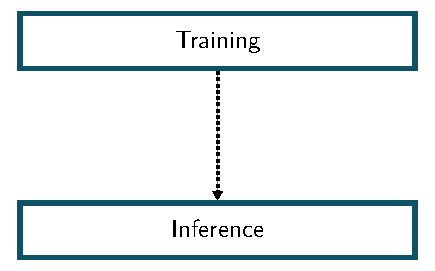
\includegraphics{ml_workflow_1.pdf}
		\subcaption{Traditional without inference optimization}\label{fig:ml-workflow-old}
	\end{minipage}%
	\begin{minipage}[b]{.5\textwidth}
		\centering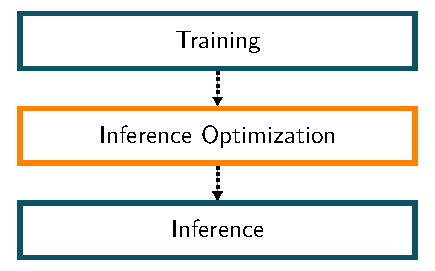
\includegraphics{ml_workflow_2.pdf}
		\subcaption{Improved with inference optimization}\label{fig:ml-workflow-new}
	\end{minipage}
	\caption[Traditional vs. optimized machine learning workflow]{Machine learning workflow}
	\label{fig:ml-workflow}
\end{figure}

The model determines what tensor operators are calculated, but it does not specify how they are calculated. Deliberately choosing the actual implementation offers great optimization potential. There is always a generic naïve implementation, which is the straightforward way of performing the calculation. However, it does not consider, e.g., memory sharing between threads or cache access patterns, which can have a significant adverse effect on performance~\cite{Hu.2017}. Techniques such as loop unrolling, reordering and tiling as well as multi-dimensional threading and tensor compute instructions can help leverage the accelerator's capabilities, but there is an abundance of combinations of settings for these techniques, the best of which is very much specific to the target device~\cite[p.~2]{Chen.2018b}. Finding the optimal such combination is the key aspect of tensor operator optimization.

Convolution operators are computationally very intensive and make up the majority of modern \glspl{cnn}, such as Inception\cite{Szegedy.2015} and ResNet\cite{He.2015}. Therefore, tensor operator optimization should focus on convolution over other types like pooling and fully-connected. It is not possible to optimize convolutions in general, but we need to optimize for every distinct parameter set that is present in the computation graph, i.e. combination of input shape, kernel shape, padding, and stride. This means that the effort increases with a higher variety of layer configurations.

\section{Manual Optimization}
Optimized implementations for tensor operators with a specific parameter set are provided by accelerator vendors in libraries like cuDNN for NVIDIA \glspl{gpu} and Intel Math Kernel Library for Intel CPUs. The vendors possess the hardware-specific knowledge to write good implementations by hand, but human expertise is required for this approach. While state-of-the-art, manual optimization has a number of inherent shortcomings:
\begin{itemize}
	\item slow support for new devices
	\item slow support for new graph-level optimizations
	\item no support for unconventional shapes
	\item vendor lock-in
\end{itemize}
These limitations hinder innovation, which is undesirable in a field so fast-evolving and relatively young as \gls{dl}. Researchers need to make a choice between avoiding devices, high-level optimizations and new network architectures that are not supported by those predefined operator libraries, and using unoptimized implementations~\cite[p.~1]{Chen.2018b}.

\section{Automated Optimization}
Automated tensor operator optimization, or \textit{autotuning}, overcomes these shortcomings by eliminating the need for human experts. Vendor-agnostic frameworks can discover good implementations regardless of hardware, model or graph optimizations. This enables innovation by fostering experimentation with novel or unconventional layers and high-level transformations that are not supported by manual libraries. Autotuning can achieve the same, in some cases even better inference performance than state-of-the-art vendor-provided operator libraries. Compared to these libraries, autotuning delivers speedups of 0.98× to 3.5× on CPU~\cite[p.~9]{Liu.2019} and 1.6× to 3.8× on server-class \glspl{gpu}~\cite[p.~10]{Chen.2018b} for commonly used \glspl{cnn}. Even a slightly worse performance is impressive considering that no domain-specific expert knowledge has been applied but only a few hours of autotuning.

Autotuning works by exploring the space of possible and functionally equivalent implementations in an iterative fashion. This \textit{search space} is defined per-operator by the set of permutations of \textit{knob} settings, which result in different implementations when being applied to a template. These knobs control, for example, loop unrolling, loop order, loop tiling and threading and can usually be adjusted in steps of powers of 2~\cite[p.~5]{Chen.2018b}~\cite[p.~16]{Vasilache.2018}. One specific combination of knob settings, i.e. one element of the search space, is called \textit{configuration}. Defining the knobs is done manually for each class of target devices, but the search is guided by an algorithm that proposes a batch of candidate configurations. This is necessary since the size of the search space makes the brute-force approach of trying all configurations infeasible. For example, the search space size for a ResNet-18 on an NVIDIA \gls{gpu} exceeds 172 million possible configurations, any one of which could be the best. \Gls{ml}-based or genetic algorithms help with rapid convergence to a decent, or ideally the best configuration without need of exhausting the whole search space.

\begin{figure}
	\begin{minipage}[b]{.45\textwidth}
		\small
		\centering
		\begin{minipage}{\textwidth}
			\begin{center}
				$ C = A^{T}B $
			\end{center}
			\unskip
			\subcaption{Mathematical expression}\label{fig:expr-sched-example-1}
		\end{minipage}
		\begin{minipage}{\textwidth}
		\begin{center}
			\bigskip
			$ C = sum(A[k, y] * B[k, x], axis=k) $
		\end{center}
		\end{minipage}
		\subcaption{Tensor index expression}\label{fig:expr-sched-example-2}
	\end{minipage}%
	\hfill
	\scriptsize
	\begin{minipage}[b]{.5\textwidth}
		\centering
		\begin{pythoncode*}{linenos=false,frame=none}
for y in range(1024):
  for x in range(1024):
    C[y][x] = 0
    for k in range(1024):
      C[y][x] += A[k][y] * B[k][x]
		\end{pythoncode*}
		\unskip
		\subcaption{Naïve schedule}\label{fig:expr-sched-example-3}
	\end{minipage}
	\begin{minipage}[b]{.45\textwidth}
		\centering
		\bigskip
		\begin{pythoncode*}{linenos=false,frame=none}
for yo in range(128):
  for xo in range(128):
    C[yo*8:yo*8+8][xo*8:xo*8+8] = 0
    for ko in range(128):
      for yi in range(8):
        for xi in range(8):
          for ki in range(8):
            C[yo*8+yi][xo*8+xi] +=
              A[ko*8+ki][yo*8+yi]
                * B[ko*8+ki][xo*8+xi]
		\end{pythoncode*}
		\unskip
		\subcaption{Tiled schedule}\label{fig:expr-sched-example-4}
	\end{minipage}
	\hfill
	\begin{minipage}[b]{.55\textwidth}
		\centering
		\bigskip
		\begin{pythoncode*}{linenos=false,frame=none}
inp_buffer AL[8][8], BL[8][8]
acc_buffer CL[8][8]
for yo in range(128):
  for xo in range(128):
    vdla.fill_zero(CL)
    for ko in range(128):
      vdla.dma_copy2d(AL, A[ko*8:ko*8+8][yo*8:yo*8+8])
      vdla.dma_copy2d(BL, B[ko*8:ko*8+8][xo*8:xo*8+8])
      vdla.fused_gemm8x8_add(CL, AL, BL)
    vdla.dma_copy2d(C[yo*8:yo*8+8,xo*8:xo*8+8], CL)
		\end{pythoncode*}
		\unskip
		\subcaption{Schedule with accelerator-specific instructions}\label{fig:expr-sched-example-5}
	\end{minipage}
	\caption[Expressions and schedules for transposed matrix multiplication]{Expressions and schedules for transposed matrix multiplication~\cite[p.~4]{Chen.2018b}}
	\label{fig:expr-sched-example}
\end{figure}

Figure \ref{fig:expr-sched-example} provides an example of how different configurations affect the generated code. The operator functionality is some mathematical calculation, in our example a transposed matrix multiplication (\ref{fig:expr-sched-example-1}). Before autotuning, that functionality is specified in a tensor expression language, which describes how to compute each element of the output tensor from the input tensors using a concise notation (\ref{fig:expr-sched-example-2}). Note that this notation is implicit, meaning that it does not prescribe implementation details. The autotuning framework then makes the computation explicit by applying the configuration to the operator's template, which lowers the tensor expression to a \textit{schedule}. A simple but naïve reference schedule can be used to check the correctness of more complex schedules (\ref{fig:expr-sched-example-3}). The schedule is an intermediate representation that allows transforms, e.g. tiling for memory locality (\ref{fig:expr-sched-example-4}) or accelerator-specific instructions for buffers and specialized tensor operators (\ref{fig:expr-sched-example-5}). The specific tiling factors and buffer sizes can be varied and are determined by the applied configuration~\cite[p.~4~ff.]{Chen.2018b}~\cite[p.~9~ff.]{Vasilache.2018}.

Since the schedule is only an intermediate representation, target-specific code, e.g., LLVM assembly for CPU or a CUDA kernel for NVIDIA \glspl{gpu}, needs to be generated. The appropriate compiler then builds that code, possibly in parallel for multiple configurations in a batch, after which the implementation can be executed. For autotuning, the execution time is then profiled on the target device to evaluate the performance. The profiling result is then stored alongside the implementation and fed back to the algorithm that selects candidate configurations. This allows the algorithm to improve its proposals for the next batch~\cite[p.~15~f.]{Vasilache.2018}. The iterative autotuning process can be stopped when a sufficiently fast implementation has been found or no better one has been discovered in a long time. Then, the full computation graph can be used for inference with the best implementations that have been found in the autotuning process for all operators.

There are two frameworks that implement autotuning, which will be described now.

\subsection{TensorComprehensions}
\glsunset{tc}
\acrlong{tc}\footnote{\url{https://github.com/facebookresearch/TensorComprehensions}} (\acrshort{tc}) has been developed by Facebook's AI Research team and comprises three main components: a language to express tensor computations (similar to Figure \ref{fig:expr-sched-example-2}), an optimizing compiler to generate efficient \gls{gpu} code from expressions, and an autotuner that finds good implementations and stores them in a compilation cache. It uses a polyhedral compiler to reason about and manipulate the loop structures of a schedule~\cite[p.~3]{Vasilache.2018}. However, only tensor-operators are considered, the framework is designed to be independent of computation graphs~\cite[p.~4]{Vasilache.2018}.

Autotuning in \gls{tc} starts from configurations that worked well for similar expressions, and some predefined strategies. The autotuner determines the configuration parameters and admissible value ranges. Then, a genetic algorithm generates a batch of candidate configurations. The value for each configuration parameter is randomly selected from one of three parents that are selected probabilistically based on their fitness. Furthermore, there is a low probability of mutation, which means that a random value is assigned to some parameters. Configurations are then compiled in parallel and profiled on an available GPU. A fitness value inversely proportional to the execution time is assigned to the configuration and stored in the autotuning database. Then, the process starts anew by selecting the next candidates using the updated database. This is repeated for a set amount of time~\cite[p.~15~f.]{Vasilache.2018}.

\subsection{TVM}
TVM\footnote{\url{https://github.com/dmlc/tvm/}} started as a research project at the University of Washington but is now supported and used by a large open-source community and companies like Amazon and Facebook. Unlike \gls{tc}, which only represents and optimizes tensor operators, TVM is an end-to-end \gls{dl} compiler stack. It can import whole models from a frontend framework and build minimal, optimized modules that can be deployed to backends like CPUs, \glspl{gpu} or FPGAs. Figure \ref{fig:tvm-stack} shows how the layers of the stack provide different levels of abstraction.

\begin{figure}
	\centering
	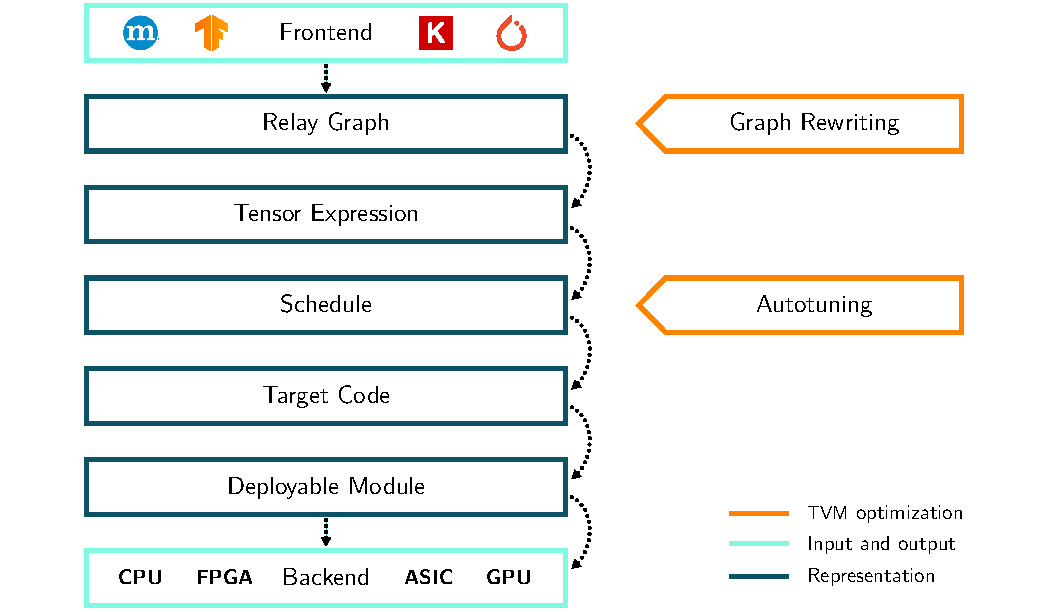
\includegraphics[width=\textwidth]{tvm_stack.pdf}%
	\caption{Levels of abstractions in TVM flow}
	\label{fig:tvm-stack}
\end{figure}

The top layer in the TVM stack is Relay. Relay is an intermediate model representation that enhances traditional computation graphs with concepts of functional programming to form a more powerful language. Relay supports shape-dependent tensor types and automatic differentiation, which is essential for \gls{dl} training~\cite[p.~61]{Roesch.2018}.  Additionally, a runtime to execute Relay programs in various programming languages is provided and needs to be present whenever executing TVM-based models. Relay programs can be created programmatically or from a textual source code. More convenient for users, however, is the import from diverse frontends, including TensorFlow, Keras, PyTorch and MXNet, which enables the use and optimization of existing models. Graph-level optimization in TVM is pass-based, with each pass inspecting or rewriting the syntax tree of the Relay program in some way. Standard passes are provided and perform, for example, automatic differentiation, type inference, operator fusion or tensor layout transformations~\cite[p.~3]{Chen.2018b}. Beyond that, writing custom passes is facilitated by an extensible design.

Next in the stack is a tensor expression language, which has similar features as \gls{tc}'s. It allows user to describe computation rules that generate a tensor without specifying loop structures and other details. The rules are composed of primitive mathematical operations like addition and multiplication, which are expressive enough to describe convolutions and other matrix and vector operations. TVM comes with tensor expressions for common computations used in \gls{dl} such as various activation functions, pooling, and linear transformation.

Lowering to schedule, then target code
calls target-specific compiler

autotuning
using machine learning


define autotuning job, task
first extraction of tasks
schedules as abstraction with knobs
details of autotuning process
Profiling repeated multiple times
Schedule intermediate representation
RPC allows autotuning logic to run on powerful server, but profiling to happen on target device
with figure
transfer learning using invariant representation
Describe saved modules

In this project, we use TVM because of the novel, machine learning-based approach
Using (commit id) with a few modifications to support measurements (check what else we changed)
